\section{The entry point}

Our Input data is a file in a \textbf{cml file}, which is a standart of xml. The file contains the information generated by the output of the experiment. It holds either MS data, or NMR data.\\
    \begin{figure}[h]
    \begin{centering}
    \caption{Example of cml file}
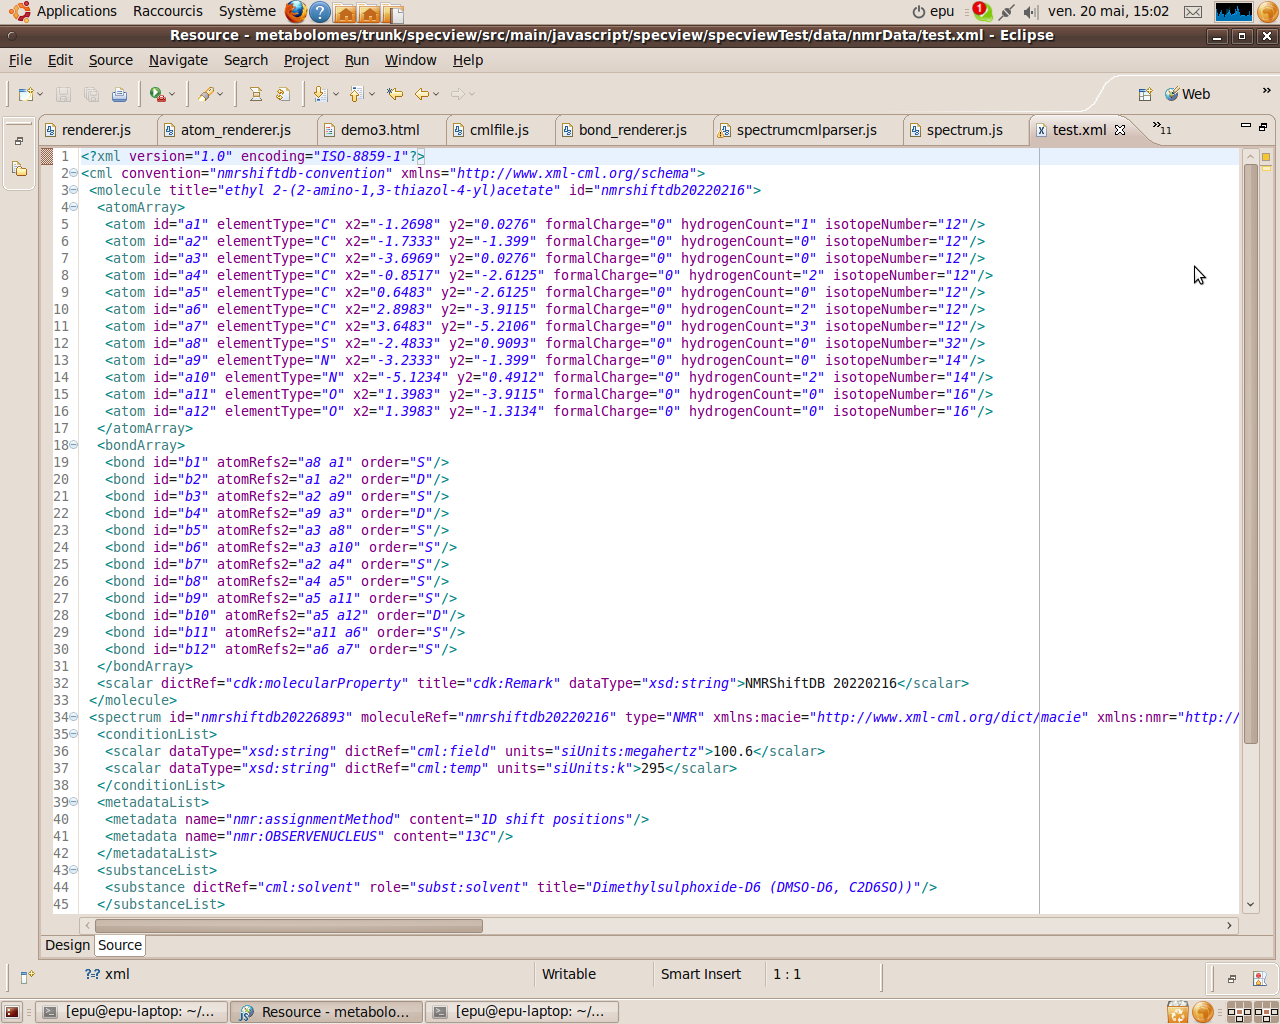
\includegraphics[width=190mm,height=160mm]{./images/sampleCML}
%    \label{subd}
    \end{centering}
    \end{figure}

\subsection{What does it contain?}

This file provides all the information required in order to build a \textbf{molecule} and a \textbf{spectrum}.
THe molecule consists in a liste of \textbf{\textit{atoms}}:
    \begin{figure}[h]
    \begin{centering}
    \caption{A list of atoms}
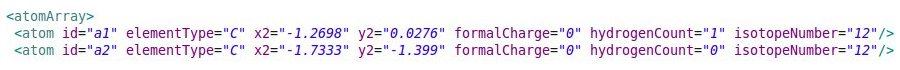
\includegraphics[width=180mm,height=13mm]{./images/atoms}
   \end{centering}
The list of atoms contains all the informations to identify the entities of the molecules. The important point is that the coordinates it contains are relative coordinates. In order to display the atoms on the screen, they have to be transformed into actual coordinates, ``pixel coordinates''.
    \end{figure}
    \begin{figure}[h]
    \begin{centering}
    \caption{A list of bonds}
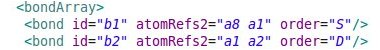
\includegraphics[width=75mm,height=7mm]{./images/bonds}
    \end{centering}
    \end{figure}
The bonds refer to 2 atoms by their id. It is possible, that single order bond have a certain stereo specificity. In that case, the bond $``b_i''$ would have a tag $``bondStereo''$ specifying the orientation of the bond.
    \begin{figure}[h]
    \begin{centering}
    \caption{Example of peak annotation for a NMR experiment}
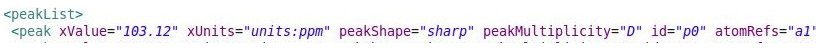
\includegraphics[width=150mm,height=10mm]{./images/annotation}
    \end{centering}
    \end{figure}
Thie information about the \textbf{peak} os probably the most important. This where the \textbf{annotation} stands. Each peak has a \textbf{\href{http://www.w3schools.com/schema/el\_field.asp}{field}} or a \textbf{\href{http://www.w3schools.com/dom/dom\_node.asp}{child}} that refer to:\\

-One or multiple \textbf{atom} if the file holds \textbf{NMR} experiment

-One or multiple \textbf{molecule} if the file holds \textbf{MS} experiment\\
The objects are mentioned by their inner identifier(identifier found in the file, e.g $a_1$,$a_2$... for an atom and $m_1$,$m_2$... for a molecule).

Furthermore, MS files can have fields tagged ``scalar information'' at the end of each molecule. These file holds additional information on the moleculem, such as physico chemical properties, inChi key, other identifiers...\\
Finally, the file contains other information regarding the experiment within the tag ``condition'' and ``metadata''.



\clearpage
